\section{Methods}
\label{sec:methods}
\begin{table}[t]
  \centering
    \renewcommand{\arraystretch}{1.2}

    \begin{tabular}{@{}llll@{}}
      \toprule
      \textbf{Callee}& \textbf{Caller} & \textbf{Module} & \textbf{Call-Site}\\ \midrule
      Basic blocks & Basic blocks & Functions & Arguments \\
      Instructions & Instructions & Instructions & Known arguments\\
      Store instructions & Store instructions & Basic blocks &  \\
      Call instructions & Call instructions & Direct calls &  \\
      Branch instructions & Branch instructions &  &  \\
      Loops & Loops &  &  \\
      Uses & Uses &  &  \\
      Influenced branches & Untouched call-sites &  &  \\
      Influenced instructions &  &  &  \\ \bottomrule 

    \end{tabular}
  \caption{RL features. \emph{Influenced instructions
      (branches)} are the those  whose operands have statically known arguments. \emph{Uses} indicates how many times the
\emph{caller} and the \emph{callee} are invoked.}
  \label{tab:features}
\end{table}

In this section, we formulate the debloating problem as a reinforcement learning
problem, describe the learning procedure, and its hyperparameters.

\paragraph{Action, state, and reward.}
To determine whether a call-site should be specialized or not, we train a policy
using reinforcement learning. This requires defining \emph{action},
\emph{state}, and \emph{reward}.

An action is whether to run a code transformation, called
\emph{specialization}, or not. Consider a call to function $\mathit{calleeF}$
with arguments $A$ at a call-site $c_i$. Let $\mathsf{formals}$ be a map from
call-site arguments to their corresponding formal parameters. Let $B$, $B
\subseteq A$, be the arguments whose values are are statically known. Then,
specialization of the call-site does: 
\begin{enumerate}
\item Create a new function $spec\_calleeF(\mathsf{formals}(A \setminus B))$,
  such that $spec\_calleeF$'s body is identical to the body of the original
  $calleeF$ except that $\mathsf{formals}(B)$ are replaced with their values.
  
\item Perform constant propagation to push forward the information to the
  rest of callee's body, potentially specializing more call-sites in
  the callee.
  
\item Replace $\mathit{calleeF}(A)$ with $spec\_calleeF(A \setminus B)$ at the
  call-site $c_i$.
\end{enumerate}

Note that after specialization, a software debloater
can trigger other optimization passes such as inlining and dead-code
elimination.

A state is a vector capturing
all the relevant information about the code. We experiment with two
state representations: (a)  a vector of hand crafted features (\textbf{\textbf{HF}}),
and (b) an embedding of LLVM IR via \insttovec (\textbf{\textbf{IV}}).

In \textbf{HF}, the state is a concatenation of four feature vectors,
summarized in Table~\ref{tab:features}. They capture relevant
information about the \emph{callee}, \emph{caller}, \emph{compilation
  unit (module)}, and \emph{call-site}. Most features are
self-explanatory, and hence, we focus only on those which are novel or
more relevant for avoiding state aliasing.
%
% capturing information about \emph{The first one} is the traditional
% approach, in which we come up with a handcrafted set of features
% based on our domain knowledge. The state we choose is a
% concatenation of $4$ feature vectors capturing information about the
% \emph{caller}, the \emph{callee}, the \emph{call-site}, and the
% \emph{compilation unit}. The features are summarized in
% Table~\ref{tab:features}.
%
The \emph{state aliasing} problem occurs when two different states
have the same representation in the RL model. In our context, our
features must distinguish between two call-sites in the same basic
block when invoking the same callee with the same arguments if one is
specialized and the other not.  In~\cite{KulkarniCWS13}, the features
\emph{InLoop} (whether a call-site is in a loop), \emph{InlineDepth}
(the current inlining depth), and \emph{currentGraphSize} (how many
instructions are there in the caller, including one added by
inlining), are used to decide inlining.  However, in our case, these
features are insufficient to prevent state aliasing.  Thus, we also
add \emph{Untouched call-sites} that counts the number of call-sites
yet to be processed. Since the call-sites are processed in a fixed
order, \emph{Untouched call-sites} is sufficient to distinguish any
two call-sites in a function.



% but in our case we
% realized that those features are not enough to prevent state aliasing: 2
% call-sites in the same basic block invoking the same callee with the same
% arguments will have the same value for these features, assuming the first
% call-site is not specialized (i.e there is no change in the caller). We use one
% addition feature to indicate the position of the call-site inside the caller: how
% many call-sites are not visited yet. Because the call-sites are visited in order,
% this feature is enough to distinguish the two call-sites.



% In this approach, the problem is how to avoid state aliasing between 2
% call-sites from the same compilation unit those have the same caller, the same callee, and the same known
% arguments.


% It is not obvious what calling context feature should be used.

% \cite{KulkarniCWS13} uses \emph{InLoop (whether a call-site is in a loop)},
% \emph{InlineDepth (the current inlining depth)}, and \emph{currentGraphSize
%   (capture the changes in the caller)}, but in our case we realized that
% those features are not enough to prevent state aliasing: 2 call-sites in the
% same basic block invoking the same callee with the same arguments will have
% the same value for these features, assuming the first call-site is not
% specialized (i.e there is no change in the caller).  We use one addition feature
% to indicate the position of the call-site  inside the caller: how many call-sites are not visited yet. Because the
% call-sites are visited in order, this feature is enough to distinguish the two
% call-sites. 

In \textbf{IV}, we use \insttovec embedding from~\cite{inst2vec}. We extract the LLVM IR
of the \emph{caller}, the \emph{callee}, and the \emph{calling context} (a window of
$n$ instructions around the call-site) as a lists of instructions. Each
instruction is embedded into a vector space using \insttovec. Additionally, we
encode the arguments at the call-site as a bitvector, in which each statically
known argument  is encoded by $1$, and an unknown argument by $0$. This
bitvector is then embedded using a different embedding matrix.
%During training, the \insttovec
%embedding is fixed while the bitvector embedding matrix is trained. 
% Ashish: Can we say more about the "bitvector is then embedded using a
% different embedding matrix"? Can the matrix be explained intuitively?
% Nham: addressed.
Finally, the \textbf{IV} state is a tuple of the above four $2$-D matrices. 
% Ashish: Is "2-D" redundant above?
Note that in this case,
the calling context of each call is explicitly represented by the IR.


%The calling context is explicit with this approach.


  


%% from GSA paper

%%%%%%%%%%%%%%%%%%%%%%%%%%%%%%%%%%%%%%%%%%%%%%%%%%%%%%%%%%%%%%%%%%%%%%%%%%%%%%%%%%%%%%%%%%%%%%%%%%%%%%%%%%%%%%%%%%%%%%%%%%%%%%%%%%%%%%%%%%%%%%%%%%%%%%%%%%%%%%%%%%%%%%%%%%%%%%%%%%%%%%%%%%%%%%%%%%%%%%%%%%%%%%%%%%%%%%%%%%%%%%%%%%%%%%%%%%%%%%%%%%%%%%%%%%%%%%%%%%%%%%%%%%%%%%%%%%%%%%%%%%%%%%%%%%%%%%%%%%%%%%%%%%%%%%%%%%%%%%%%%%%%%%%%%%%%%%%%%%%%%%%%%%%%%%%%%%%%%%%%%%%%%%%%%%%%%%%%%%%%%%%%%%%%%%%%%%%%%%%%%%%%%%%%%%%%%%%%%%%%%%%%%%%%%%%%%%%%%%%%%%%%%%%%%%%%%%%%%%%%%%%%%%%%%%%%%%%%%%%%%%%%%%%%%%%%%%%%%%%%%%%%%%%%%%%%%%%%%%%%%%%%%%%%%%%%%%%%%%%%%%%%%%%%%%%%%%%%%%%%%%%%%
% Code Reuse Attacks: Code reuse attacks are a class of attacks in which an attacker compromises the control flow of a pro-gram and redirects execution to an existing executable part of the  program  to cause  a  malicious  effect,  bypassing  code in-jection  defensessuch  as  Write  XOR  Execute.In  gadget-based code reuse attack methods such as ROP, JOP, and COP [7, 21, 8, 9], the attacker chains together short instruction se-quences  called  gadgets present  in  the  program  in  a  specific order to construct a malicious payload without injecting code. %
%%%%%%%%%%%%%%%%%%%%%%%%%%%%%%%%%%%%%%%%%%%%%%%%%%%%%%%%%%%%%%%%%%%%%%%%%%%%%%%%%%%%%%%%%%%%%%%%%%%%%%%%%%%%%%%%%%%%%%%%%%%%%%%%%%%%%%%%%%%%%%%%%%%%%%%%%%%%%%%%%%%%%%%%%%%%%%%%%%%%%%%%%%%%%%%%%%%%%%%%%%%%%%%%%%%%%%%%%%%%%%%%%%%%%%%%%%%%%%%%%%%%%%%%%%%%%%%%%%%%%%%%%%%%%%%%%%%%%%%%%%%%%%%%%%%%%%%%%%%%%%%%%%%%%%%%%%%%%%%%%%%%%%%%%%%%%%%%%%%%%%%%%%%%%%%%%%%%%%%%%%%%%%%%%%%%%%%%%%%%%%%%%%%%%%%%%%%%%%%%%%%%%%%%%%%%%%%%%%%%%%%%%%%%%%%%%%%%%%%%%%%%%%%%%%%%%%%%%%%%%%%%%%%%%%%%%%%%%%%%%%%%%%%%%%%%%%%%%%%%%%%%%%%%%%%%%%%%%%%%%%%%%%%%%%%%%%%%%%%%%%%%%%%%%%%%%%%%%%%%%%%%%
For rewards, we focus on two different metrics. First, we measure the
number of instructions in the final binary produced by the software debloater
after specialization took place. Second, we measure the reduction of the
\emph{attack surface}, focusing on code reuse attacks.

\emph{Code reuse attacks} are exploits in which an attacker makes use of the
available instructions in the binary to chain together short sequences called
\textit{gadgets}, and use those gadgets to compromise the control flow of the
program, causing a malicious effect. Those sequences are often categorized based
on their last instruction, into ROP (return-oriented programming), JOP
(jump-oriented programming), and COP (call-oriented programming) gadgets,
respectively. Since the relationship between the number of gadgets and
exploitability is an open question~\cite{gsa}, we focus on reducing the number
of gadgets without making any further claim about the security of the debloated~code.

The rewards are the negations of the number of instructions, ROP, JOP, and COP
gadgets. The negation is necessary because we are interested in minimizing our
metrics. We only have one measurement at the end of an episode (when the final
binary is produced). Immediate rewards after each action are set to zero.
\paragraph{Learning procedure, policy network, and hyper-parameters.}
Each state representation requires a different neural net for the policy network.
%
For \textbf{HF}, we use a $3$-layer fully connected network. Before training, we run the
pipeline with a random policy $100$ times to calculate the mean and standard
deviation of each feature, and use this metadata to normalize all features into
mean of $0$ deviation of $1$.

For \textbf{IV}, we run the \emph{caller}, the \emph{callee}, the \emph{calling context}
and the \emph{arguments bitvector} through four separate $2$-layer
GRU~\cite{gru} blocks, concatenate the last hidden outputs of these $4$ blocks,
and then feed it to a $3$-layer fully connected network. The architecture is
depicted in Fig.~\ref{fig:inst2vec_occam}.

Both networks use ReLU~\cite{relu} as the activation function. 
% Ashish: Should a citation be added for ReLU above?
We use \reinforce~\cite{reinforce} with normalized rewards to update
the policy for both models. At each \reinforce iteration, we roll out
$k$~runs of the current policy, batch them together, and use the Adam
optimizer~\cite{adam} to update the network. For all metrics, we use the same
hyper-parameters: \insttovec calling
context $n = 10$, number of runs in each policy rollout $k =75$, Adam's learning rate = $0.001$, and train up to $340$ iterations.

     \begin{figure}
         \centering
         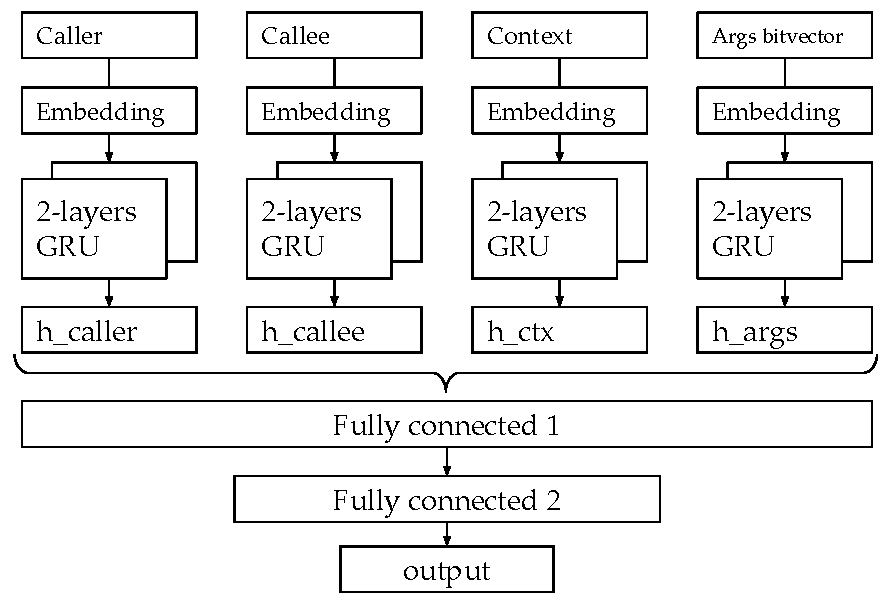
\includegraphics[width=0.75\textwidth]{doccam_figures/inst2vec_occam.pdf}
         \caption{Policy network architecture using \insttovec .}
         \label{fig:inst2vec_occam}
     \end{figure}
     \begin{figure}
         \centering
         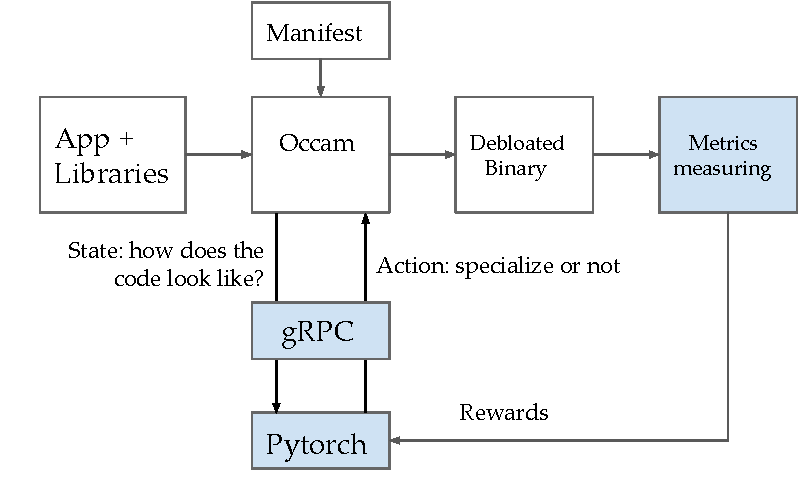
\includegraphics[width=0.75\textwidth]{doccam_figures/D-OCCAM.pdf}
         \caption{\doccam architecture. Boxes in blue correspond to this work.}
         \label{fig:d-occam}
     \end{figure}


%%% Local Variables:
%%% mode: latex
%%% TeX-master: "neurips_2019"
%%% End:

%%% Local Variables:
%%% mode: latex
%%% TeX-master: "neurips_2019"
%%% End:
